\documentclass{beamer}
\usepackage[utf8]{inputenc}
\usepackage[spanish]{babel}
\usepackage{graphicx}
\usepackage{booktabs}
\usepackage{ragged2e}
\usepackage{xcolor}
\definecolor{LightGray}{gray}{0.975}
\definecolor{links}{HTML}{2A1B81}
%\usepackage[urlcolor=blue]{hyperref}
\hypersetup{colorlinks,linkcolor=,urlcolor=blue}

\usepackage{tikz}
\usetikzlibrary{arrows,shapes}

\usepackage{algorithm}
\usepackage{algorithmic}

\usepackage{minted}
\usepackage{xcolor}
\definecolor{LightGray}{gray}{0.975}

\usepackage{listings}

%\usetheme{Warsaw}
\usefonttheme{serif}

\title[Performance Tuning]{Database Administration}
\subtitle{Lecture 08: Performance Tuning.}
\author{Valeja and Gonzales.}
\date{\today}

\setbeamertemplate{navigation symbols}{}%remove navigation symbols

\defbeamertemplate*{footline}{shadow theme}
{%
  \leavevmode%
  \hbox{\begin{beamercolorbox}[wd=.5\paperwidth,ht=2.5ex,dp=1.125ex,leftskip=.3cm plus1fil,rightskip=.3cm]{author in head/foot}%
    \usebeamerfont{author in head/foot} Database Administration \hfill \insertshorttitle
  \end{beamercolorbox}%
  \begin{beamercolorbox}[wd=.5\paperwidth,ht=2.5ex,dp=1.125ex,leftskip=.3cm,rightskip=.3cm plus1fil]{title in head/foot}%
    \usebeamerfont{title in head/foot} \hfill \insertframenumber\,/\,\inserttotalframenumber%
  \end{beamercolorbox}}%
  \vskip0pt%
}

\AtBeginSection[]
{
     \begin{frame}<beamer>
     \frametitle{Plan}
     \tableofcontents[currentsection]
     \end{frame}
}

\newcommand{\toRight}[1]{
    \begin{FlushRight}
        {\tiny #1}
    \end{FlushRight}
} % Align to right

\begin{document}

\frame{\titlepage}

\begin{frame}{Database Administration: Performance Tuning.}
    \centering
    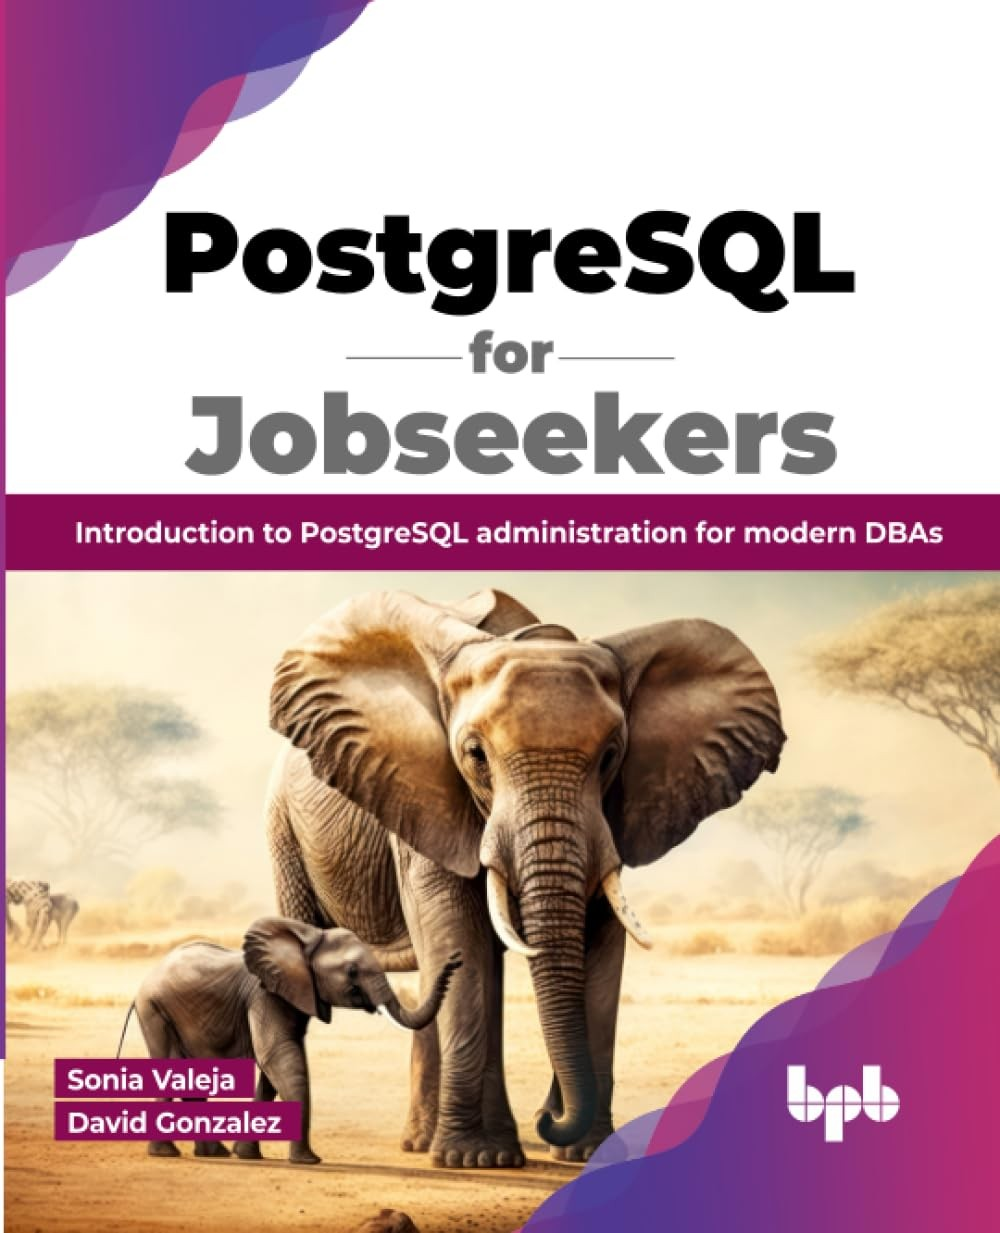
\includegraphics[width=0.4\textwidth]{figures/book_cover}\\
    \vspace{2mm}
    {
        \scriptsize
        Content has been extracted from \textit{PostgreSQL for Jobseekers (Chapter 13)}, by Sonia Valeja and David Gonzales, 2023.  Visit \url{https://bpbonline.com/products/postgresql-for-jobseekers}.\\
    }
\end{frame}

% Introduction
\begin{frame}{Introduction}
    \begin{itemize}
        \item PostgreSQL aims to resolve queries as quickly as possible.
        \item Performance tuning is a critical aspect of database administration.
        \item This presentation covers key topics including indexes, statistics, query planning, and best practices.
    \end{itemize}
\end{frame}

% Indexes
\begin{frame}{Indexes}
    \begin{itemize}
        \item Indexes help locate data efficiently, similar to a book index.
        \item Types of indexes:
        \begin{itemize}
            \item B-tree (default, supports range queries)
            \item Hash (optimized for equality comparisons)
            \item GiST and SP-GiST (used for geometric data)
            \item GIN (for arrays and full-text search)
            \item BRIN (efficient for large datasets with ordered values)
        \end{itemize}
    \end{itemize}
\end{frame}

% Reindexing
\begin{frame}{Reindexing}
    \begin{itemize}
        \item Rebuilding an index can help maintain performance.
        \item Command: \texttt{REINDEX INDEX <index-name>}
        \item Use \texttt{CONCURRENTLY} to rebuild without locking writes.
    \end{itemize}
\end{frame}

% Statistics
\begin{frame}{Statistics in PostgreSQL}
    \begin{itemize}
        \item PostgreSQL collects statistics to optimize query execution.
        \item Key system catalogs:
        \begin{itemize}
            \item \texttt{pg\_class}: stores number of rows and disk usage.
            \item \texttt{pg\_stats}: contains column value distribution statistics.
            \item \texttt{pg\_statistics\_ext\_data}: extended statistics.
        \end{itemize}
        \item Running \texttt{ANALYZE} updates statistics.
    \end{itemize}
\end{frame}

% EXPLAIN PLAN
\begin{frame}{EXPLAIN PLAN}
    \begin{itemize}
        \item Used to analyze query execution plans.
        \item Syntax: \texttt{EXPLAIN ANALYZE <query>}
        \item Helps identify if indexes are used or if sequential scans occur.
    \end{itemize}
\end{frame}

% Best Practices
\begin{frame}{Best Practices for Performance Tuning}
    \begin{itemize}
        \item Adjust key parameters in \texttt{postgresql.conf}:
        \begin{itemize}
            \item \texttt{shared\_buffers}: Set to 15-25\% of RAM.
            \item \texttt{work\_mem}: Allocate sufficient memory for sorting.
            \item \texttt{effective\_cache\_size}: Set to 50-75\% of RAM.
            \item \texttt{autovacuum}: Ensure it is enabled for table maintenance.
        \end{itemize}
        \item Regularly analyze and vacuum tables.
        \item Use indexes strategically to avoid unnecessary overhead.
    \end{itemize}
\end{frame}

% Conclusion
\begin{frame}{Conclusion}
    \begin{itemize}
        \item Proper indexing and statistics ensure efficient queries.
        \item Use \texttt{EXPLAIN ANALYZE} to evaluate query performance.
        \item Tune PostgreSQL settings based on workload needs.
    \end{itemize}
\end{frame}

\begin{frame}{Database Administration: Backup and Restore.}
    \centering
    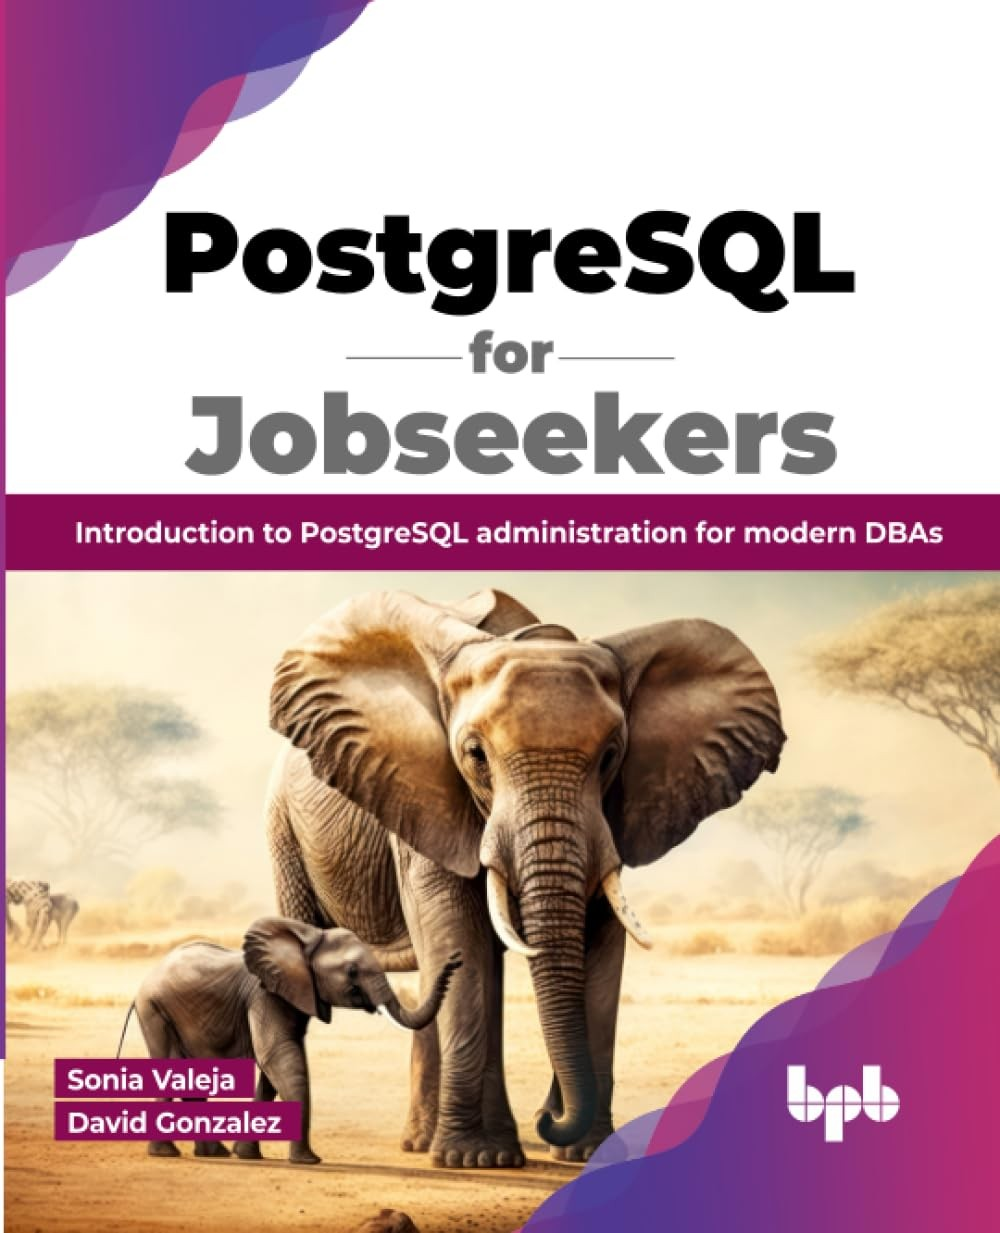
\includegraphics[width=0.4\textwidth]{figures/book_cover}\\
    \vspace{2mm}
    {
        \scriptsize
        Content has been extracted from \textit{PostgreSQL for Jobseekers (Chapter 13)}, by Sonia Valeja and David Gonzales, 2023.  Visit \url{https://bpbonline.com/products/postgresql-for-jobseekers}.\\
    }
\end{frame}

\end{document}
